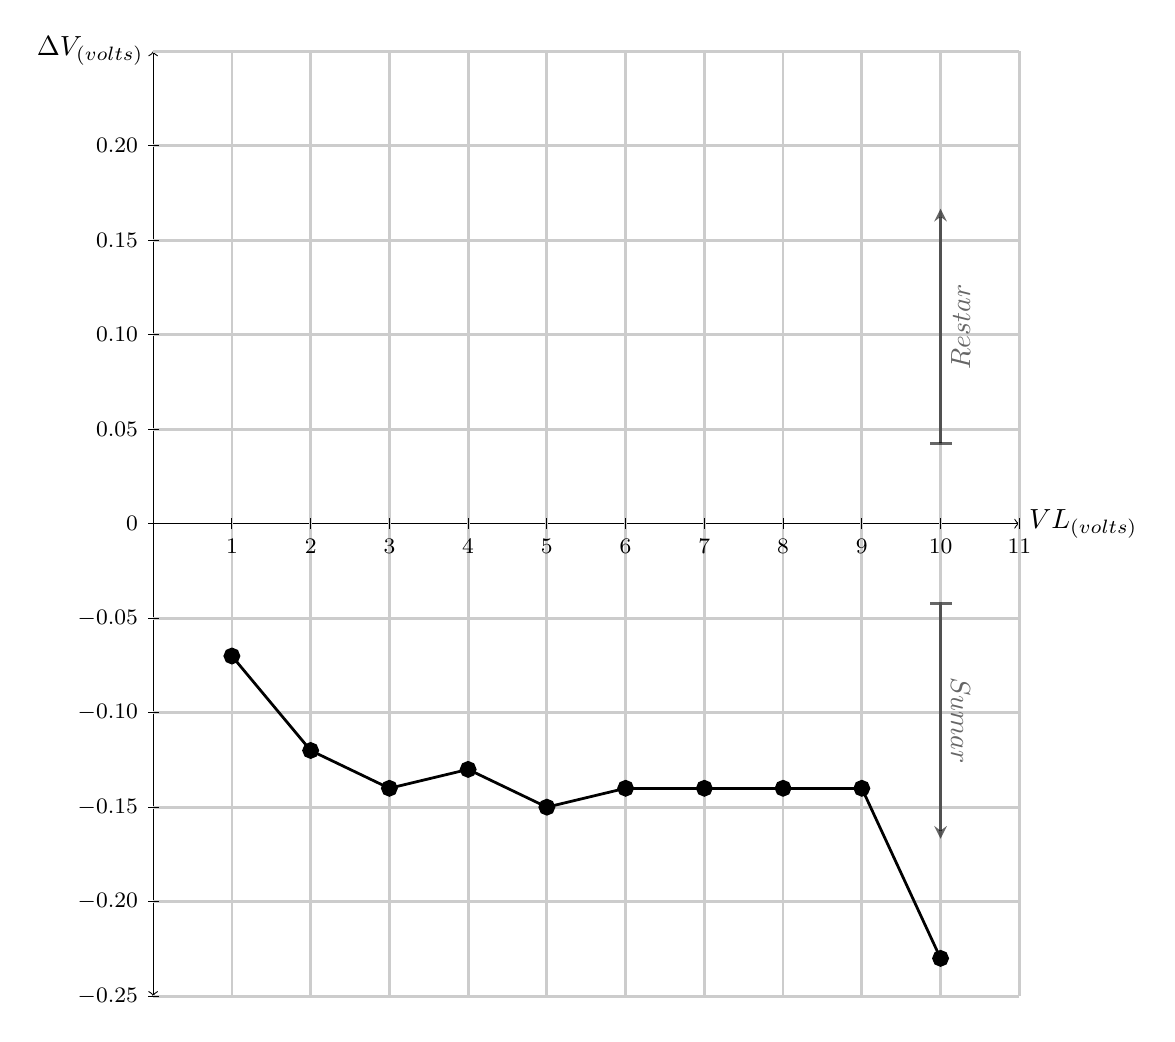
\begin{tikzpicture}[scale=1]
    
    \def\scal{6/0.25}
    
    %datosLineaA
    \coordinate (a1) at (1,-0.07*\scal);
    \coordinate (a2) at (2,-0.12*\scal);
    \coordinate (a3) at (3,-0.14*\scal);
    \coordinate (a4) at (4,-0.13*\scal);
    \coordinate (a5) at (5,-0.15*\scal);
    \coordinate (a6) at (6,-0.14*\scal);
    \coordinate (a7) at (7,-0.14*\scal);
    \coordinate (a8) at (8,-0.14*\scal);
    \coordinate (a9) at (9,-0.14*\scal);
    \coordinate (a10) at (10,-0.23*\scal);

    
    %Ejex
    \draw[->] (0,0)--(11,0) node[right] {$VL_{(volts)}$};
    \foreach \x in {1,2,...,11}{
        \draw[line width=1pt,gray!40] (\x,-6)--(\x,6);
        \draw[shift={(\x,0)}] (0pt,2pt) -- (0pt,-2pt) node[below] {\footnotesize $\x$};
    }
    %Ejey
    \draw[<->] (0,-6)--(0,6) node[left]{$\Delta V_{(volts)}$};;
    \foreach \y in {-0.25,-0.20,-0.15,-0.10,-0.05,0.05,0.10,0.15,0.20}{
        \draw[line width=1pt,gray!40] (0,\y*6/0.25)--(11,\y*6/0.25);
        \draw[shift={(0,\y*6/0.25)}] (2pt,0pt) -- (-2pt,0pt) node [left] {\footnotesize $\y$} ;
    }
   \draw[shift={(0,0)}] (2pt,0pt) -- (-2pt,0pt) node [left] {\footnotesize $0$} ;
   \draw[line width=1pt,gray!40] (0,6)--(11,6);
   
    %Linea A
    \foreach \x  in {1,...,10}{
        \draw[line width=2pt,fill=black] (a\x) circle(2pt);
   }
   \foreach \x [evaluate={\y=int(\x+1);}] in {1,...,9}{
        \draw[line width=1pt,black] (a\x) -- (a\y);
   }
   \draw[line width=1pt,opacity=0.6,|-stealth] (10,-1)--(10,-4) node[midway,sloped,above]{$Sumar$};
   \draw[line width=1pt,opacity=0.6,|-stealth] (10,1)--(10,4) node[midway,sloped,below]{$Restar$};
   
\end{tikzpicture}

